\documentclass{book}
\usepackage{amssymb,amsmath}
\usepackage{polyglossia}
\setmainlanguage{spanish} % Idioma principal
\usepackage{theorem}
\usepackage{times}
\usepackage{array}
\usepackage{graphicx}
\usepackage{hyperref}
\usepackage{multirow}
\usepackage{fancyhdr}
%\usepackage[cp1252]{inputenc}
\usepackage{hhline}
\usepackage{multicol}
\usepackage[a4paper,driver=xetex,top=4.5cm,head=4.5cm, bottom=2cm,%
layouthoffset=0mm, left=2.5cm, right=2.5cm,marginparwidth=0cm]{geometry}
%\usepackage{bm}
%\usepackage{tabular}
\usepackage{fontspec}
 \usepackage[breakable,many]{tcolorbox}
\defaultfontfeatures{Ligatures=TeX}
\usepackage{empheq}
 \setromanfont{Oswald-Light}
 \usepackage{float}
 \usepackage{mathrsfs} 
%
%
% \renewcommand{\familydefault}{\sfdefault}
%\renewcommand{\familydefault}{\sfdefault}

%%%%%%%%%Estilo de la pagina%%%%%%%%%%%%%%%%%%%%%%%%%%%%%%%%%%%
%%%%%%%%%%%%%%%%%%%%%%%%%%%%%%%%%%%%%%%%%%%%%%%%%%%%%%%%%%%%%%%%%%
% \newcounter{ejer}
% 
% {\theorembodyfont{\normalfont}
% \newtheorem{ejercicio}[ejer]{Ejercicio}}

\newcommand{\rr}{\mathbb{R}}
\newcommand{\qq}{\mathbb{Q}}
\newcommand{\nn}{\mathbb{N}}



\DeclareMathOperator{\atan2}{atan2}
%\DeclareMathOperator{\sen}{sen}
\DeclareMathOperator{\sign}{sign}
\DeclareMathOperator{\sn}{sn}
\DeclareMathOperator{\SO}{SO}
%\DeclareMathOperator{\arcsen}{arcsen}
\DeclareMathOperator{\Or}{O}

\usepackage[framemethod=TikZ]{mdframed}
%%%%%%%%%%%%%%%%%%%%%%%%%%%%%%
%Theorem

%% Ejercicio
\newcounter{ejer} \setcounter{ejer}{0}
\renewcommand{\theejer}{\arabic{ejer}}
\newenvironment{ejer}[2][]{%
\vspace{5pt}
\refstepcounter{ejer}%
\ifstrempty{#1}%
{%
% \mdfsetup{%
% frametitle={%
% \tikz[baseline=(current bounding box.east),outer sep=-0pt]
% \node[anchor=east,rectangle,fill=green!50]
{\noindent\bfseries Ejercicio~\theejer}.}
%
{%
% \mdfsetup{%
% frametitle={%
% \tikz[baseline=(current bounding box.east),outer sep=0pt]
% \node[anchor=east,rectangle,fill=green!50]
{\noindent\bfseries  Ejercicio~\theejer:~#1};}%
%
%\mdfsetup{innertopmargin=10pt,linecolor=green!50,%
%linewidth=2pt,topline=true,%
%frametitleaboveskip=\dimexpr-\ht\strutbox\relax
%}
%\begin{mdframed}[]
\relax%
\label{#2}}{\vspace{5pt}}%\end{mdframed}}

%Theorem
\newcounter{theo}[chapter] \setcounter{theo}{0}
\renewcommand{\thetheo}{\arabic{section}.\arabic{theo}}
\newenvironment{theo}[2][]{%
\refstepcounter{theo}%
\ifstrempty{#1}%
{\mdfsetup{%
frametitle={%
\tikz[baseline=(current bounding box.east),outer sep=0pt]
\node[anchor=east,rectangle,fill=blue!20]
{\strut Teorema~\thetheo};}}
}%
{\mdfsetup{%
frametitle={%
\tikz[baseline=(current bounding box.east),outer sep=0pt]
\node[anchor=east,rectangle,fill=blue!20]
{\strut Teorema~\thetheo:~#1};}}%
}%
\mdfsetup{innertopmargin=10pt,linecolor=blue!20,%
linewidth=2pt,topline=true,%
frametitleaboveskip=\dimexpr-\ht\strutbox\relax
}
\begin{mdframed}[]\relax%
\label{#2}}{\end{mdframed}}
%%%%%%%%%%%%%%%%%%%%%%%%%%%%%%
%Lemma
\newcounter{lem}[chapter] \setcounter{lem}{0}
\renewcommand{\thelem}{\arabic{section}.\arabic{lem}}
\newenvironment{lem}[2][]{%
\refstepcounter{lem}%
\ifstrempty{#1}%
{\mdfsetup{%
frametitle={%
\tikz[baseline=(current bounding box.east),outer sep=0pt]
\node[anchor=east,rectangle,fill=green!20]
{\strut Lemma~\thelem};}}
}%
{\mdfsetup{%
frametitle={%
\tikz[baseline=(current bounding box.east),outer sep=0pt]
\node[anchor=east,rectangle,fill=green!20]
{\strut Lemma~\thelem:~#1};}}%
}%
\mdfsetup{innertopmargin=10pt,linecolor=green!20,%
linewidth=2pt,topline=true,%
frametitleaboveskip=\dimexpr-\ht\strutbox\relax
}
\begin{mdframed}[]\relax%
\label{#2}}{\end{mdframed}}
%%%%%%%%%%%%%%%%%%%%%%%%%%%%%%
%% Definicion
\newcounter{defini}[chapter] \setcounter{defini}{1}
\renewcommand{\thedefini}{\arabic{section}.\arabic{defini}}
\newenvironment{definicion}[2][]{%
\refstepcounter{defini}%
\ifstrempty{#1}%
{\mdfsetup{%
frametitle={%
\tikz[baseline=(current bounding box.east),outer sep=0pt]
\node[anchor=east,rectangle,fill=green!20]
{\strut Definición~\thedefini};}}
}%
{\mdfsetup{%
frametitle={%
\tikz[baseline=(current bounding box.east),outer sep=0pt]
\node[anchor=east,rectangle,fill=green!20]
{\strut Definición~\thedefini:~#1};}}%
}%
\mdfsetup{innertopmargin=10pt,linecolor=green!20,%
linewidth=2pt,topline=true,%
frametitleaboveskip=\dimexpr-\ht\strutbox\relax
}
\begin{mdframed}[]\relax%
\label{#2}}{\end{mdframed}}

%Proof
\newenvironment{prf}{\noindent\emph{Dem.}}{$\square$ \newline\vspace{5pt}}


%Corolario
\newcounter{cor}[chapter] \setcounter{cor}{0}
\renewcommand{\thecor}{\arabic{section}.\arabic{cor}}
\newenvironment{cor}[2][]{%
\refstepcounter{cor}%
\ifstrempty{#1}%
{\mdfsetup{%
frametitle={%
\tikz[baseline=(current bounding box.east),outer sep=0pt]
\node[anchor=east,rectangle,fill=green!20]
{\strut Corolario~\thelem};}}
}%
{\mdfsetup{%
frametitle={%
\tikz[baseline=(current bounding box.east),outer sep=0pt]
\node[anchor=east,rectangle,fill=green!20]
{\strut Corolario~\thelem:~#1};}}%
}%
\mdfsetup{innertopmargin=10pt,linecolor=green!20,%
linewidth=2pt,topline=true,%
frametitleaboveskip=\dimexpr-\ht\strutbox\relax
}
\begin{mdframed}[]\relax%
\label{#2}}{\end{mdframed}}

\tcbset{highlight math style={enhanced,
  colframe=red!60!black,colback=yellow!50!white,arc=4pt,boxrule=1pt,
  drop fuzzy shadow}}
  
  
  
  
  
  
  


\pagestyle{fancyplain}

 \renewcommand{\sectionmark}[1]
                 {\markright{\thesection\ #1}}


% \lhead[\fancyplain{}{\bfseries\thepage}]
%       {\fancyplain{}{\bfseries\rightmark}}
%
 \rhead[\fancyplain{}{\bfseries\leftmark}]{\fancyplain{}{\bfseries}}




 \lhead[\fancyplain{}{ 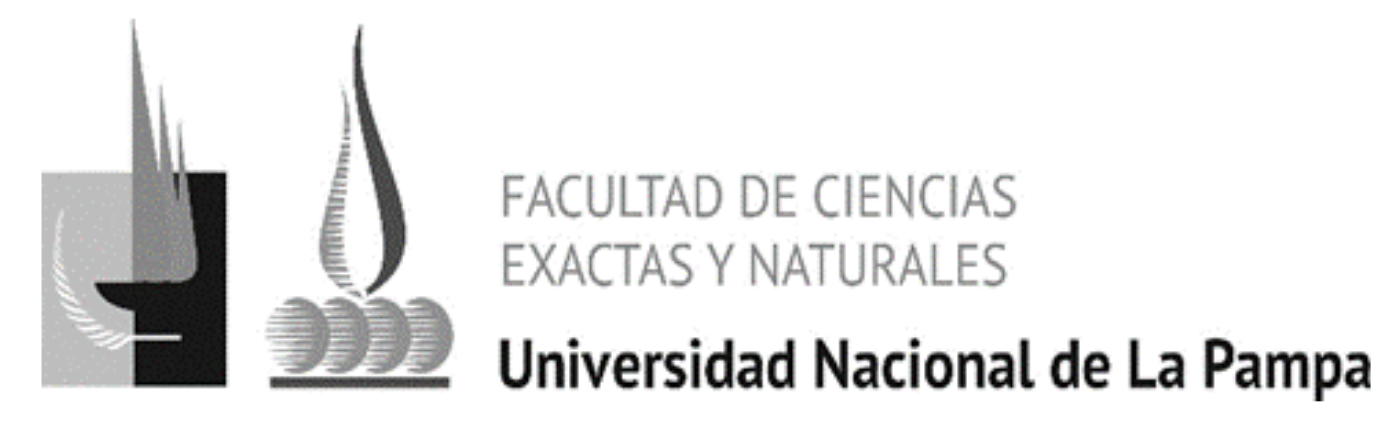
\includegraphics[scale=.3]{EscudoUNLPam.png}}]{\fancyplain{}{ 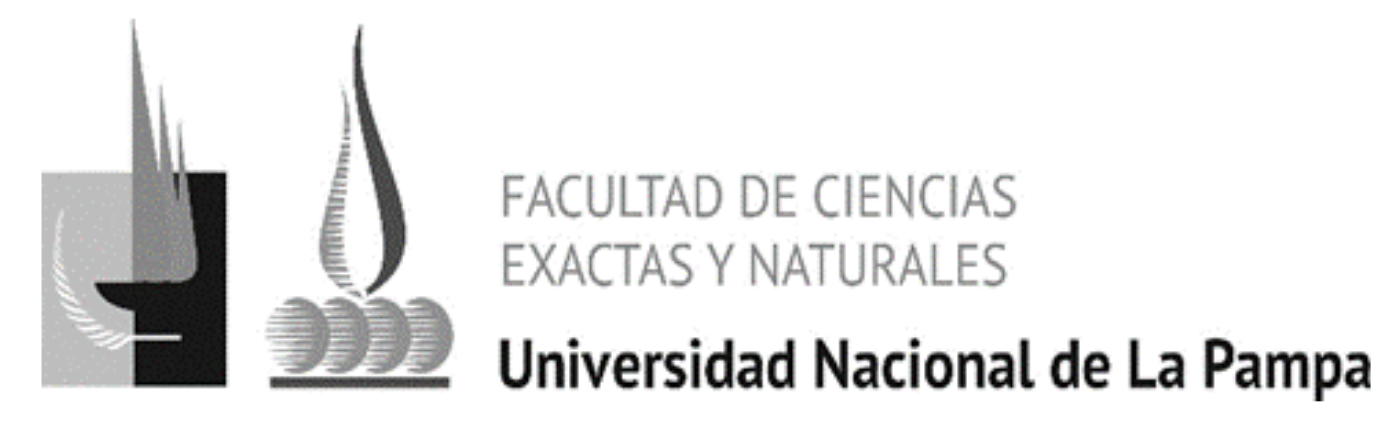
\includegraphics[scale=.3]{EscudoUNLPam.png}}}

\cfoot{}





  
  
  
  
  
  
  
\begin{document}


\hyphenation{excen-tri-ci-dad}


\begin{large}
\begin{bfseries} % \begin{scshape}
        \noindent Depto de Matem\'atica.\\
        Primer Cuatrimestre de 2022\\                                                                                                                                                                                                                                                                                                                                                
        Teoría de la Medida \\
        Práctica 1: Cardinalidad

%\end{scshape}
\end{bfseries}
\end{large}
\par\noindent\rule{\textwidth}{.5pt}

\begin{ejer}{} Sea $f:A\longrightarrow B$ una función cualquiera.
Supongamos que $\{A_i\}_{i\in I}$ y $\{B_i\}_{i\in I}$ son
familias subindicadas de conjuntos, donde los $A_i$ y $B_i$ son
subconjuntos de $A$ y $B$ respectivamente. Demostrar las
siguientes propiedades:

\begin{itemize}
\item[1.] $\biggl(\bigcup_{i\in I}A_i\biggr)^c=\bigcap_{i\in
I}A_i^c$.
\item[2.]$\biggl(\bigcap_{i\in I}A_i\biggr)^c=\bigcup_{i\in
I}A_i^c$.
\item[3.] $f\biggl(\bigcup_{i\in I}A_i\biggr)=\bigcup_{i\in
I}f(A_i)$.
\item[4.]?`Qué ocurre con $f\biggl(\bigcap_{i\in I}A_i\biggr)$?
\item[5.] $f^{-1}\biggl(\bigcup_{i\in I}B_i\biggr)=\bigcup_{i\in
I}f^{-1}(B_i)$.
\item[6.]$f^{-1}\biggl(\bigcap_{i\in I}B_i\biggr)=\bigcap_{i\in
I}f^{-1}(B_i)$.
\end{itemize}
\end{ejer}

\begin{ejer}{3}  Demostrar que si $f:A\longrightarrow B$ una función, entonces
\begin{itemize}
\item[1.] $f(C_1\cup C_2)=f(C_1)\cup f(C_2).$
\item[2.]$f^{-1}(D_1\cup D_2)= f^{-1}(D_1)\cup f^{-1}(D_2).$
\item[3.] $f(C_1\cap C_2)\subset f(C_1)\cap f(C_2).$ Dar un ejemplo de que la igualdad no vale en general.
\item[4.]$f^{-1}(D_1\cap D_2)= f^{-1}(D_1)\cap f^{-1}(D_2).$
\end{itemize}
\end{ejer}

\begin{ejer}{1} Probar que $\thicksim$ es una
relación de equivalencia.
\end{ejer}

\begin{ejer}{1.2} Supongamos que $A\thicksim B$ y
$C\thicksim D$.
\begin{itemize}
\item[1.] Demostrar que $\mathscr{P}(A)\thicksim \mathscr{P}(B)$.
\item[2.] Demostrar que $A\times C\thicksim B\times D$.
\item[3.] Demostrar que $A^C\thicksim B^D$.
\item[4.] Si $A\precsim C$ entonces $B\precsim D$.
\item[5.] Si $A\precsim B$ entonces $A^C\precsim B^C$.

\end{itemize}
\end{ejer} 

\begin{ejer}{1.5} \textbf{*} Demostrar que un subconjunto de un conjunto
finito es finito.
\end{ejer}

\begin{ejer}{2} Demostrar que la función
$f:\nn\times\nn\longrightarrow\nn$ definida por:
\[f(j,k):=\frac{(j+k-1)(j+k)}{2}-j+1,\]
es una biyección.
\end{ejer}

\begin{ejer}{} Encontrar, de manera explícita, una cantidad numerable de subconjuntos
de $\nn$, mutuamente disjuntos y cada uno de ellos 
numerable. Usar esto para dar otra demostración de que $\nn\times\nn$ es
numerable.
\end{ejer}

\begin{ejer}{5} Demostrar, exhibiendo una biyección, que $(0,1)\thicksim [0,1]$
\end{ejer}



\begin{ejer}{8} Demostrar que, para cualquier conjunto
$A$, $\mathscr{P}(A)\thicksim\{0,1\}^A$.
\end{ejer}

\begin{ejer}{infcoordconsub} Demostrar que son
equivalentes:
\begin{itemize}
     \item[1.] $A$ es infinito.
     \item[2.] $A$ es coordinable con un subconjunto propio, es
     decir: Existe $B\subset A$, con $B\neq A$, tal que
     $A\thicksim B$.
\end{itemize}
\end{ejer}

\begin{ejer}{}\textbf{*} Sea $A$ un conjunto infinito y $B\subset A$ 
 numerable. Supongamos que $A-B$ es infinito. Demostrar que
$A-B\sim A$.
\end{ejer}




\begin{ejer}{} Sean $A$ y $B$ conjuntos y supongamos que existe
una función  $f$ de $A$ en $B$ suprayectiva. Demostrar que $\#
B\leq \#A$.
\end{ejer}

\begin{ejer}{} Demostrar que el conjunto formado por todos los
subconjuntos de $\nn$ que son finitos, es numerable.
?`Qué ocurrira con el conjunto de todos los subconjuntos
infinitos?
\end{ejer}

\begin{ejer}{}\textbf{*}  Sea $\{A_i\}_{i\in I}$ una familia de intervalos
de $\rr$. Suponer que los conjuntos en la familia son mutuamente
disjuntos, es decir: $A_i\cap A_j=\emptyset$ si $i\neq j$.
Demostrar que el conjunto $\{A_i:i\in I\}$ es a lo sumo numerable.
\end{ejer}

\begin{ejer}{}\textbf{*}  Recordemos que una función
$f:\rr\longrightarrow\rr$ se dice nodecre-\newline ciente, si para
todos $x,y\in\rr$, tales que $x<y$, se tiene que $f(x)\leq f(y)$.
Dada una función nodecreciente, demostrar que el conjunto de
todos los puntos de discontinuidad es a lo sumo numerable.
\textit{Ayuda}: Demostrar en primera instancia que los
límites laterales:
\[
    \lim\limits_{x\rightarrow a^+}f(x)\quad\text{y}\quad \lim\limits_{x\rightarrow
    a^-}f(x)
\]
existen para todo $a\in\rr$. Luego aplicar el ejercicio anterior.
\end{ejer}

\begin{ejer}{} Demostrar que $\rr^{\nn}\thicksim\rr$ ($c^{\aleph_0}=c$).
\end{ejer}

\begin{ejer}{}\textbf{*}  Como aprendimos $\nn\thicksim\mathbb{Q}$, esto
significa que existe una aplicación biyectiva
$f:\nn\longrightarrow\mathbb{Q}$, que nos permite enumerar
$\mathbb{Q}$ como una suceción $r_j:=f(j)$. Definimos la
aplicación:
\[\begin{split}
              T:C(\rr)&\longrightarrow \rr^{\nn}\\
              f        &\longmapsto T_f\\
\end{split}\]
donde
\[
  T_f(j):=f(r_j).
\]
\begin{itemize}
   \item [1.] Demostrar que $T$ es inyectiva. Por consiguiente
   $C(\rr)\precsim\rr^{\nn}$.
   \item[2.] Usando el inciso anterior, demostrar que
    $C(\rr)\thicksim\rr$, donde $C(\rr)$ es el conjunto
    de las funciones continuas de $\rr$ en si mismo.
\end{itemize}
\end{ejer}



\end{document}
